\chapter{How to install and load packages in R}
\label{cha:install-load-packages}

To know how to install packages, the first thing is to know what R packages we already have installed. This can be known with the commands shown in Listing \ref{cod:installed-packages}. Both of two commands show a list of installed packages.

\begin{codefloat}
\begin{lstlisting}[language=R, style=Ccolor]
installed.packages()
library()
\end{lstlisting}
\caption{Commands to show installed packages.}
\label{cod:installed-packages}
\end{codefloat}

To install a new package, we only need to know its name. We also can search the package in \href{https://cran.r-project.org/}{CRAN R project} website. There, click on \textbf{Packages} in the menu on the left and search for the desired package either ordered by date of publication (Table of available packages, sorted by date of publication) or ordered by name (Table of available packages, sorted by name). These steps can be seen in Figure \ref{fig:cran-website} and \ref{fig:packages-by-name}.

\begin{figure}[H]
  \begin{subfigure}[b]{0.39\textwidth}
    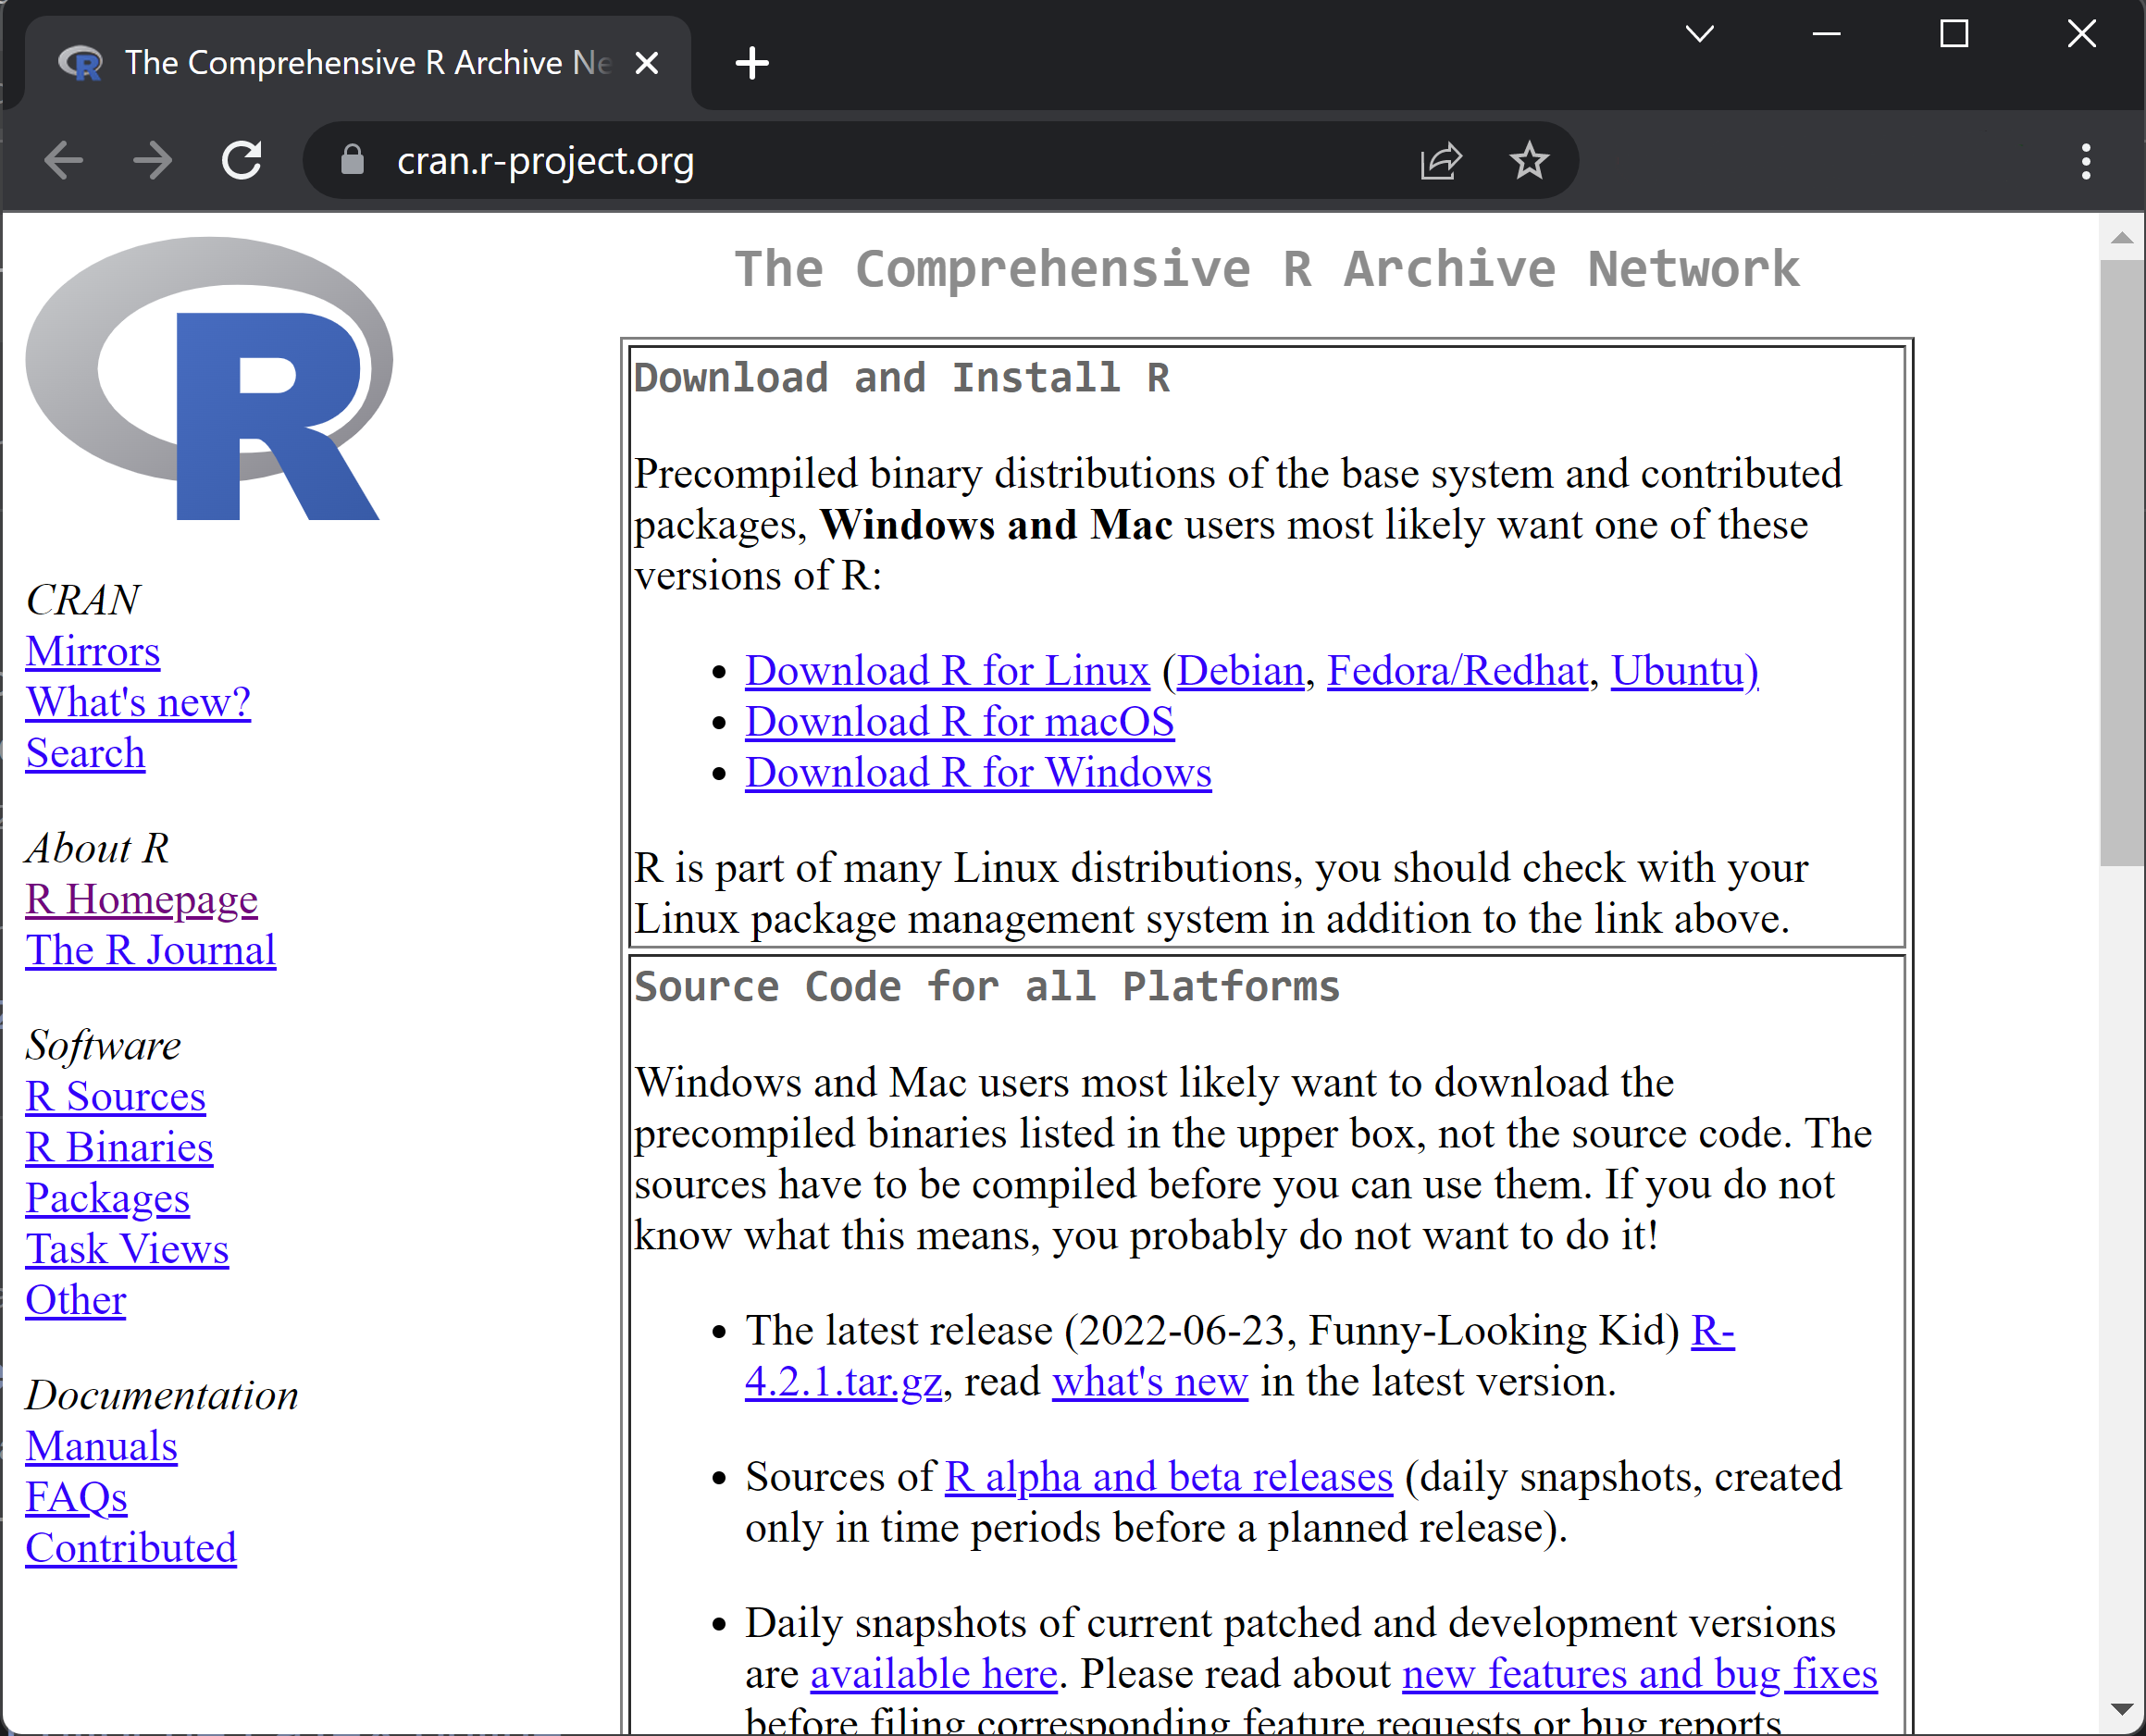
\includegraphics[scale=1.5]{installing-packages-r/cran.png}
    \caption{CRAN menu.}
    \label{fig:cran-menu}
  \end{subfigure}
  \hfill
  \begin{subfigure}[b]{0.59\textwidth}
    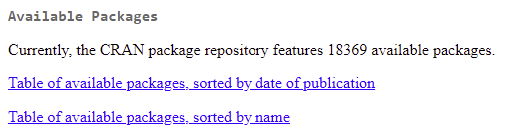
\includegraphics[scale=1.5]{installing-packages-r/cran2.png}
    \caption{\textbf{Packages} option.}
    \label{fig:packages-option}
  \end{subfigure}
  \caption{\acrshort{cran} left menu and Available Packages section}
  \label{fig:cran-website}
\end{figure}
\begin{figure}[H]
    \centering
    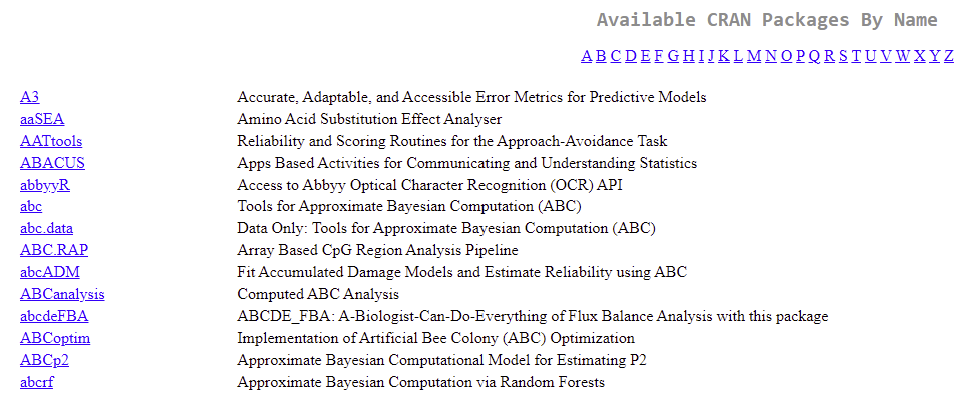
\includegraphics[scale=1.4]{installing-packages-r/cran3.png}
    \caption{Packages sorted by name.}
    \label{fig:packages-by-name}
\end{figure}

Then you just have to use install.packages() function with the name of the package that you want to install between quotes as a parameter. The dplyr package will be installed to show as an example. See Listing \ref{cod:install-packages-example}.

\begin{codefloat}
\begin{lstlisting}[language=R, style=Ccolor]
install.packages("dplyr")
\end{lstlisting}
\caption{Example of install.packages() function to install dplyr package.}
\label{cod:install-packages-example}
\end{codefloat}

When the installation is finished, the package is at your local library. In order to use the package it has to be found in the R standard library. The standard library is the library that the R Foundation considers to be the most important set of packages, the most used, and the most commonly used. The standard library is loaded by default when R is loaded to make it easier to work with. To query the packages that are available to load in the standard library, use library() without any arguments. It is the same command used in Listing \ref{cod:installed-packages} because the packages installed and those ready to be loaded into the standard library are the same. To check what packages are loaded, use search(). See Listing \ref{cod:search}.

\begin{codefloat}
\begin{lstlisting}[language=R, style=Ccolor]
search()
 [1] ".GlobalEnv"  "tools:rstudio"  "package:stats"  "package:graphics"  "package:grDevices"  "package:utils"    
 [7] "package:datasets"  "package:methods"  "Autoloads"  "org:r-lib"  "package:base"  
\end{lstlisting}
\caption{search() execution.}
\label{cod:search}
\end{codefloat}

To load the package from your local library to the standard library, you also use library() but with the name of the package you want to load as a parameter. Remember to load the package again to use it if you open a new session in R or RStudio. Only the default standard library packages are loaded automatically. See a load example in Listing \ref{cod:library}.

\begin{codefloat}
\begin{lstlisting}[language=R, style=Ccolor]
library(dplyr)  
\end{lstlisting}
\caption{Load dplyr package with library().}
\label{cod:library}
\end{codefloat}

Now the package is ready to be used.

You can also install a package from a GitHub repository, such as DefectData, a package used to load the datasets used in this project. To do this you need to first install the devtools package (see Listing \ref{cod:devtools}). This package offers tools to make developing R packages easier and it contains a function that is very useful to install from GitHub, install\_github().

\begin{codefloat}
\begin{lstlisting}[language=R, style=Ccolor]
install.packages("devtools") 
\end{lstlisting}
\caption{Install devtools package.}
\label{cod:devtools}
\end{codefloat}

To use the mentioned function, instead of loading the devtools package with library(), as explained above, you can mention the package and call the function directly using ::. The name of the repository to be installed is passed as a parameter. See Listing \ref{cod:install-github}.

\begin{codefloat}
\begin{lstlisting}[language=R, style=Ccolor]
devtools::install_github("klainfo/DefectData")
\end{lstlisting}
\caption{Install from GitHub with install\_github().}
\label{cod:install-github}
\end{codefloat}

Finally, an R script has been created with all the R packages used during the development of this project. This script is shown in Listing \ref{cod:installation.R}.

\begin{codefloat}[b]
\lstinputlisting[language=R, style=Ccolor]{listings/installation.R}
\caption{R script to install all necessary packages.}
\label{cod:installation.R}
\end{codefloat}